%!TEX root = Report.tex
\chapter{Resultate und Diskussion}\label{sec:results}

Die Messergebnisse in Abbildung \ref{pic:figure1} und Abbildung \ref{pic:figure2} zeigen deutlich, dass die berechnete Gastemperatur ($T_{gas}$) weit unter den gemessenen Temperaturen $T_1$ und $T_2$ liegt und somit $\dot Q_{conv}$ stets negativ ist. $\dot Q_{conv} < 0$ bedeutet das Gas nimmt Wärme von der Lanze auf, bzw. diese wird vom Gas gekühlt.

\begin{figure}[H]
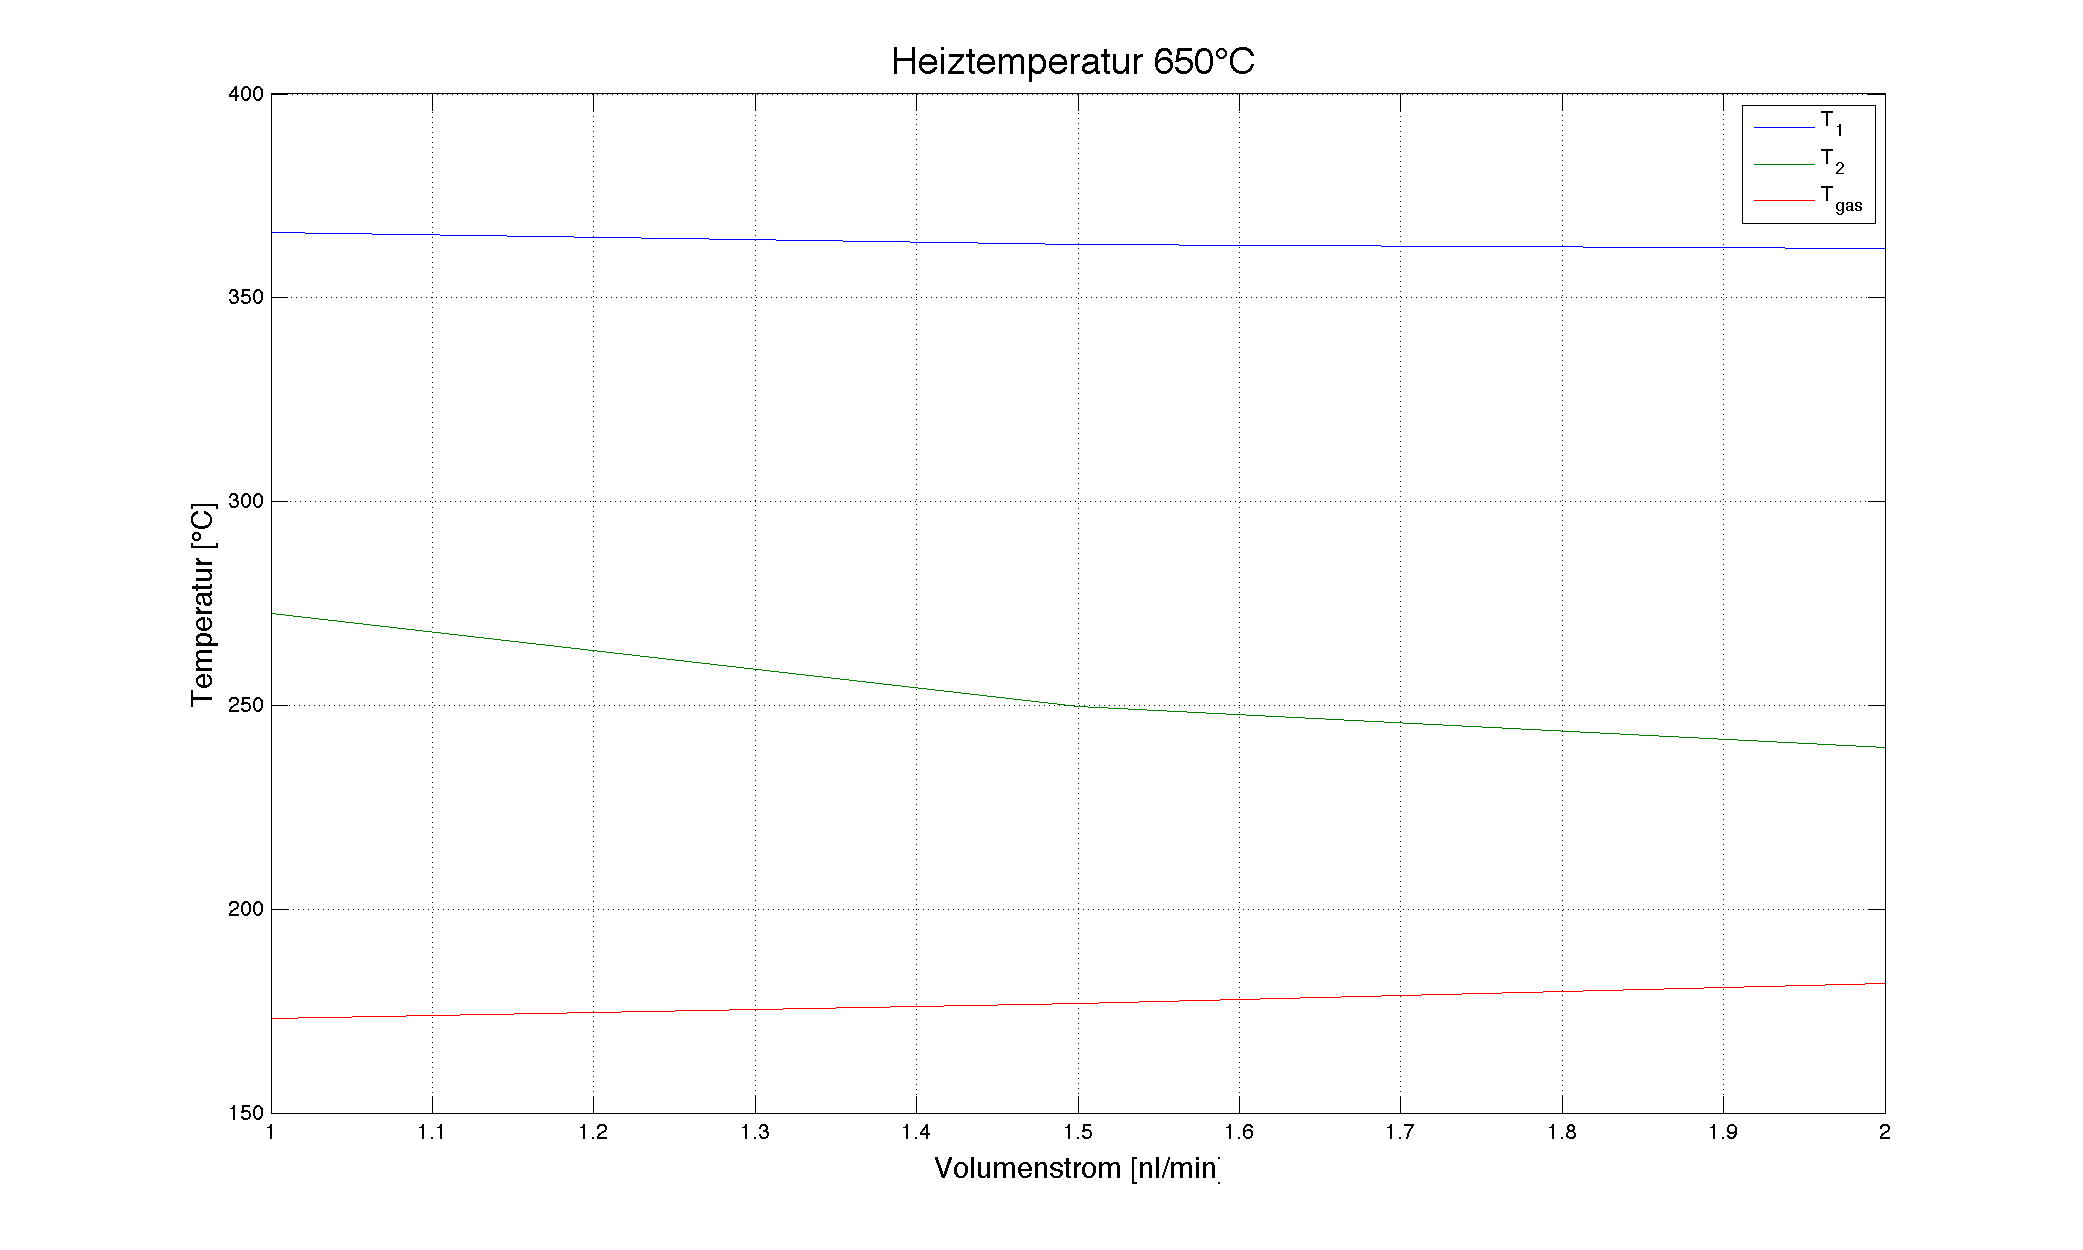
\includegraphics[width=\textwidth]{pics/figure1.png}
\caption{Messresultate bei $T= 650^\circ C$}
\label{pic:figure1}
\end{figure}

Ausserdem ist es offensichtlich, dass  höhere Temperaturen eine  grössere Verfälschung zwischen gemessenem und berechneten Wert verursachen, da die Wärmestrahlung mit der vierten Potenz der Temperatur zunimmt und die Messung des Thermoelements beeinflusst.\\

Des Weiteren ist zu beobachten dass die Temperatur $T_1$ in beiden Messreihen annährend konstant bleibt, obwohl der Volumenstrom zunimmt. Dies ist auch durch den grossen Einfluss der Wärmestrahlung des Rohrofens zu erklären, welche unabhängig vom Volumenstrom des Gases ist. Zudem spürt das Thermoelement, welches $T_1$ misst, nur einen kleinen konvektiven Wärmeübergang, welcher durch das Absaugen kaum beeinflusst wird. 

\begin{figure}[H]
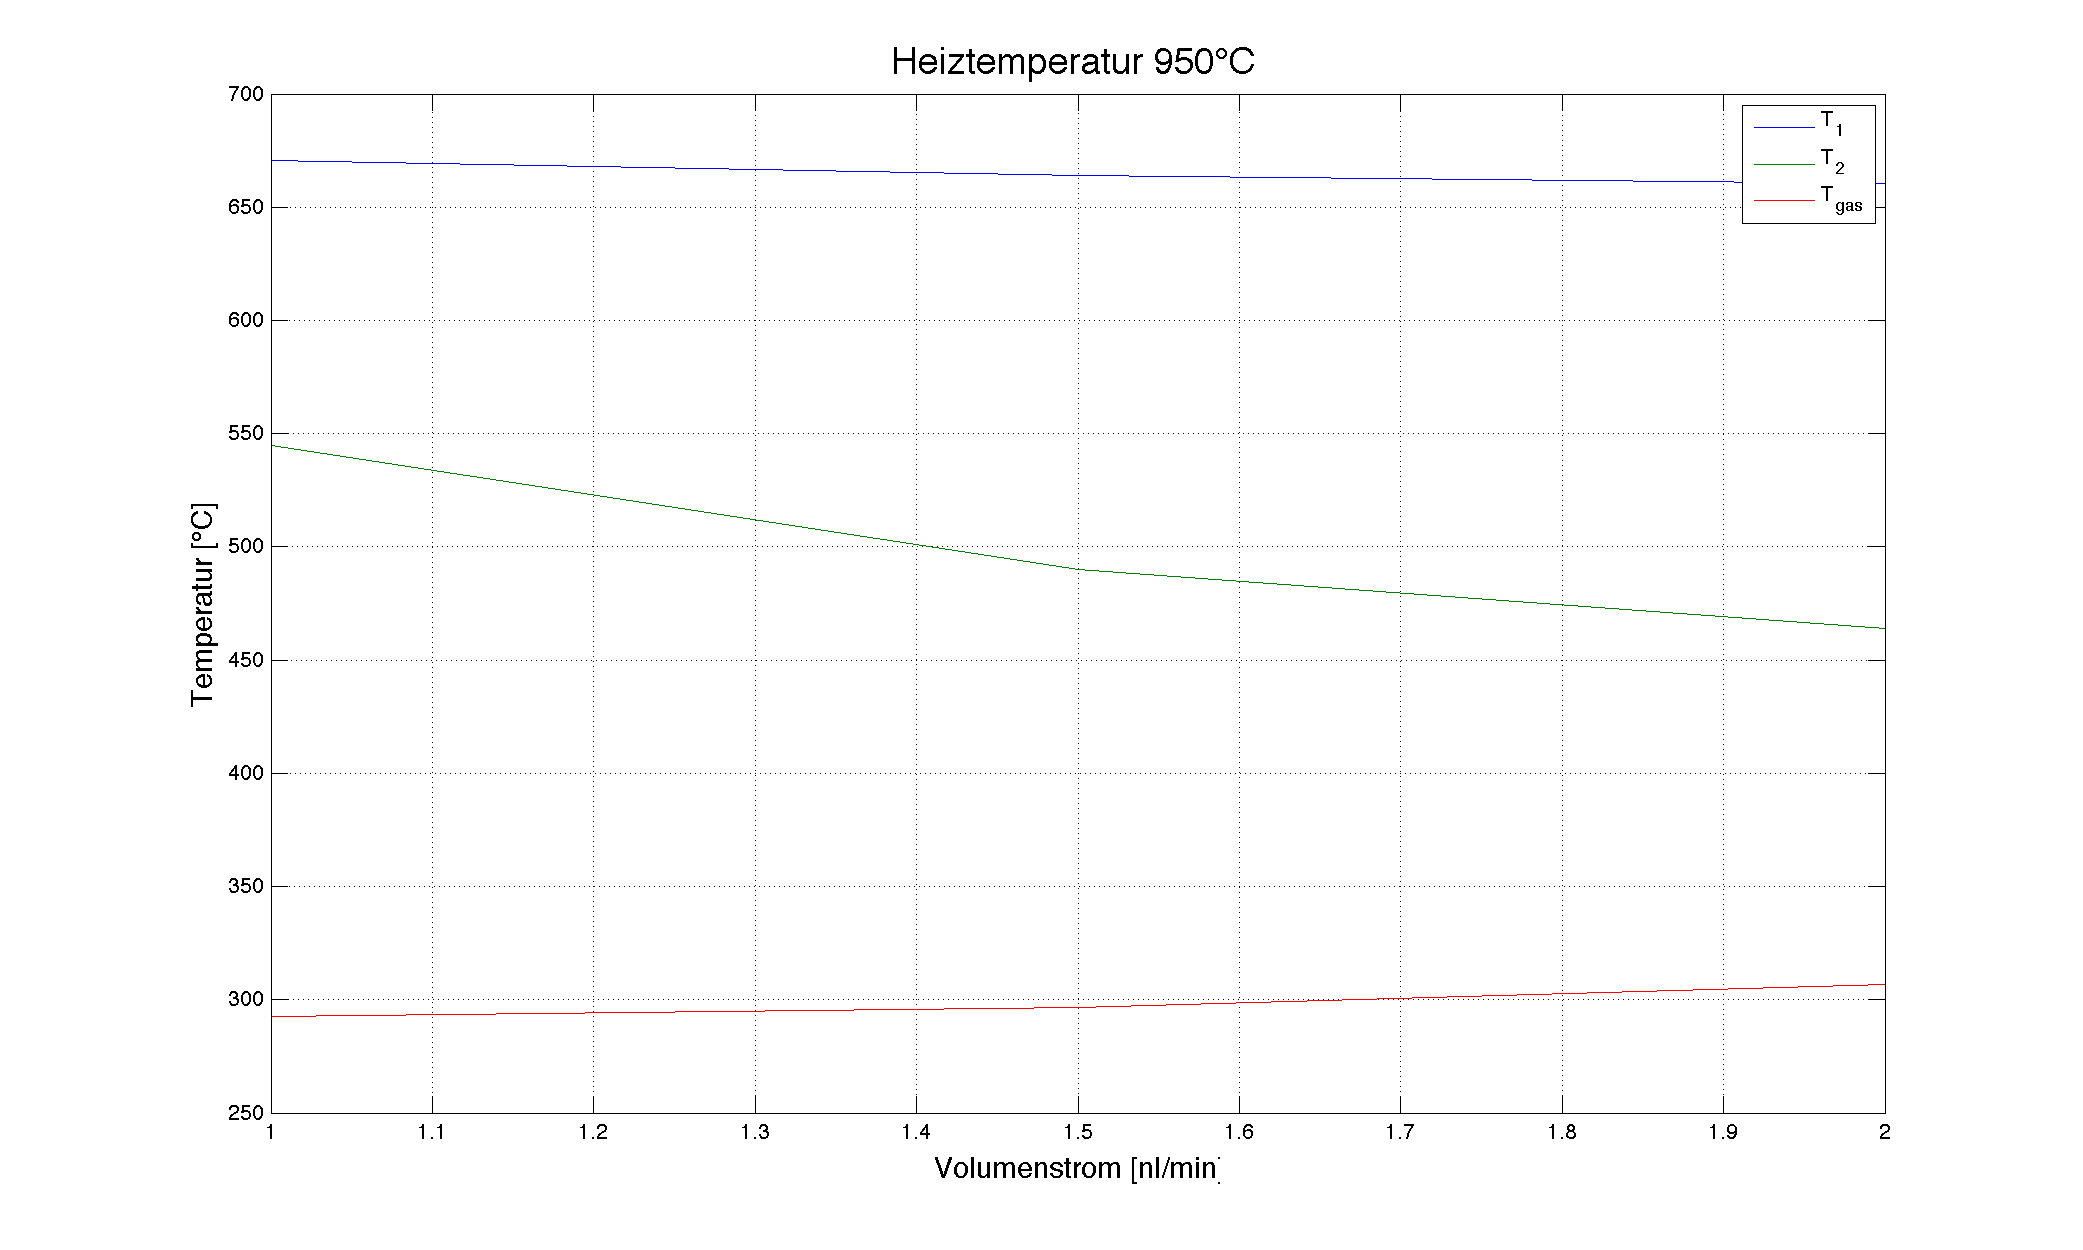
\includegraphics[width=\textwidth]{pics/figure2.png}
\caption{Messresultate bei $T= 950^\circ C$}
\label{pic:figure2}
\end{figure}



Im Fall von $T_2$ spielt der konvektive Wärmeübergang des Gases eine nicht zu vernachlässigende Rolle. Hier fällt die gemessene Temperatur mit zunehmendem Volumenstron ab, da der erzwungene konvektive Wärmeübergang grösser wird und die Gastemperatur konstant bleibt.\\




